\documentclass[11pt,aspectratio=169]{beamer}

\usepackage{amssymb}
\usepackage{physics}
% \DeclareMathOperator{\Tr}{Tr}

\title{Torus amplitudes and modular invariance}
\date[16.5.2022]{Seminar on Theoretical Physics}
\author{Otto T.P. Schmidt}
%\institute[Organizational Unit]{Organizational Unit\\can spread over 2 lines}
\institute[Department of Physics]{}
\usetheme{eth}

\colorlet{titlefgcolor}{ETHblue}
\colorlet{accentcolor}{ETHred}

\begin{document}

%\def\titlefigure{elements/title-page-image}		% Default image
%\def\titlefigure{elements/title-page-image-43}	% Use this for 4:3 presentations

\titleframe

% \colorlet{titlefgcolor}{ETHpurple}
% \def\titlefigure{elements/title-page-image-alt}
% \title{Different background}
% \titleframe

% \colorlet{titlefgcolor}{ETHgreen}
% \colorlet{titlebgcolor}{ETHgreen!60!black}
% \def\titlefigure{}
% \setlength{\titleboxwidth}{0.75\textwidth}			% Change box width
% \title{Or even a plain color, especially if your title is very long and leaves no space for what's behind the colored box}
% \titleframe

\tocframe

\section{Motivation}

\begin{frame}[fragile]{\underline{Interactions and observables}}

	In the study of string interactions, the ultimate goal will be the assignment of a probability for a certain process and the prediction of a physical cross section.
	\\~\\
	As outlined in Section 22, the computation of an observable cross section involves a series of steps:
	\begin{enumerate}
		\item Canonical representation of string diagram through moduli space
		\item Compute scattering amplitude by means of conformal field theory
		\item Convert scattering amplitude into a cross section
	\end{enumerate}
	
	
		




\end{frame}

\begin{frame}[fragile]{\underline{Loop amplitudes in string theory}}
	
	In order to obtain accurate scattering amplitudes of processes,
	one needs to include contributions from loops in string diagrams. 
	\\~\\
	These loops can be seen as contributions
	from the next higher order pertubation. 
	Graphically we consider the following processes:
	\begin{figure}[htbp]
		\centering
		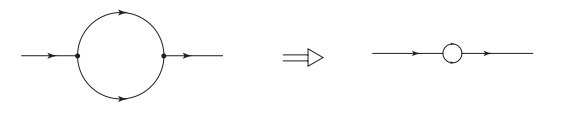
\includegraphics[width = 0.55\textwidth]{elements/Feynman loop}
	\end{figure}


\end{frame}

\begin{frame}{\underline{Ultraviolet divergence}}

	Amplitudes from virtual processes as depicted before can lead to ultraviolet (UV) divergences in quantum field theory (QFT).
	\\~\\
	Whereas QFT must employ complex renormalizations to deal with these UV divergences, we do not encounter these problems in string theory.
	
\end{frame}



\section{The moduli space of tori}

\subsection{One-loop open strings}

\begin{frame}[fragile]{\underline{One-loop open strings}}

	Before approaching the moduli space of tori, lets consider a one-loop open string with light-cone momentum $p^{+}$. This will serve as an intuitive analogon.

	The light-cone diagram is:
	\begin{figure}[htbp]
		\centering
		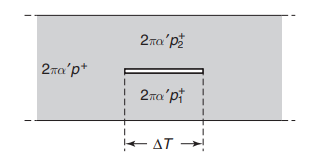
\includegraphics[width = 0.45\textwidth]{elements/one-loop open string.PNG}
	\end{figure}

	For fixed external momentum $p^+$ we find the two parameters: $\Delta T \in (0, \infty)$ and $p_{1}^{+} \in (0, p^+)$.
	\\
	$\rightarrow$ The class of Riemann surfaces of this process has two moduli.

\end{frame}

\begin{frame}{\underline{Canonical annulus}}

	Use $w = \tau + i \sigma$ and apply conformal transformations:
	\\~\\
	\begin{enumerate}
		\item Exponential map: $z = exp[\frac{w}{2 \alpha^{'} p^+}]$
		\item Linear fractional transformation: $\eta = \frac{1+iz}{1-iz}$
		% \item Canonical annulus: \textit{A region in} \mathbb{C} \textit{that is topologically an annulus can be mapped conformally to a canonical annulus}
		\item Canonical annulus: \textit{A region in $\mathbb{C}$ that is topologically an annulus can be mapped conformally to a canonical annulus}

	\end{enumerate}

	\begin{columns}
		\begin{column}{0.25\textwidth}
			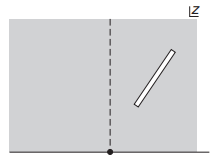
\includegraphics[width=\columnwidth]{elements/exponential map.PNG}
		\end{column}
		\begin{column}{0.25\textwidth}
			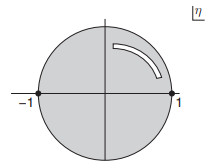
\includegraphics[width=\columnwidth]{elements/LFT.PNG}
		\end{column}
		\begin{column}{0.25\textwidth}
			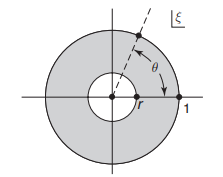
\includegraphics[width=\columnwidth]{elements/canonical annulus.PNG}
		\end{column}
	\end{columns}
	
\end{frame}

\subsection{Rectangular tori}

\begin{frame}{\underline{Rectangular tori}}

	In order to apply the concept of moduli spaces to a torus, we need to assure that a torus is indeed a Riemann surface.
	\\
	Consider a rectangular region of $\mathbb{C}$. By applying the analytic identifications $z \sim z + L_1$ and $z \sim z + iL_2$
	we obtain a torus. This shows that the region remains a Riemann surface. 
	\\
	Graphically:
	\begin{columns}
		\begin{column}{0.25\textwidth}
			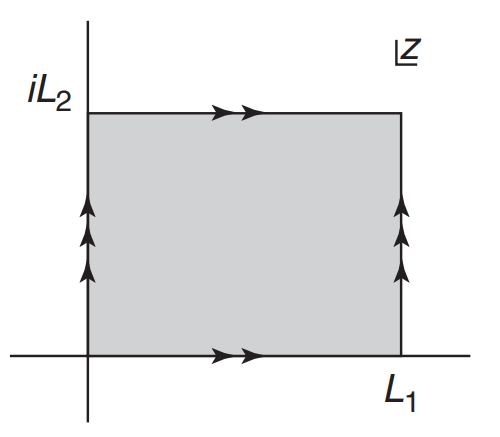
\includegraphics[width=\columnwidth]{elements/region C.PNG}
		\end{column}
		\begin{column}{0.2\textwidth}
			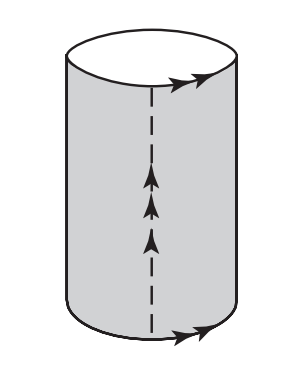
\includegraphics[width=\columnwidth]{elements/first ident.PNG}
		\end{column}
		\begin{column}{0.25\textwidth}
			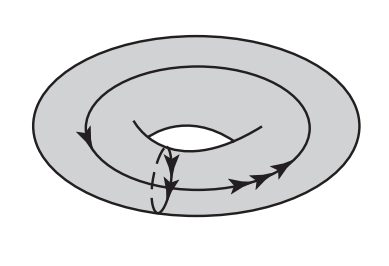
\includegraphics[width=\columnwidth]{elements/second ident.PNG}
		\end{column}
	\end{columns}


	
\end{frame}

\begin{frame}{\underline{Parametrisation}}

	We have:
	\\
	\begin{block}{Rectangular torus}
		$z \sim z + L_1$ and $z \sim z + iL_2$
	\end{block}
	\bigskip
	By applying $z^{'} = \frac{z}{L_1}$ the identifications become:
	\begin{block}{Torus parameter T}
		$z^{'} \sim z^{'} + 1$ and $z^{'} \sim z^{'} + iT$ with $T = \frac{L_2}{L_1}$
	\end{block}

\end{frame}

\begin{frame}{\underline{Ultraviolet divergence}}

	T is a parameter of the torus but does not yet define the moduli space, i.e. tori with different T can be conformally equivalent.
	\\
	Consider the following series of conformal maps to a rectangular torus with $T<1$:

	\begin{figure}[htbp]
		\centering
		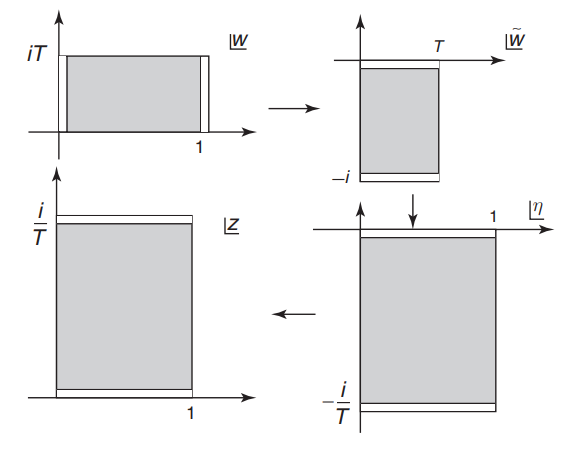
\includegraphics[width = 0.30\textwidth]{elements/three maps.PNG}
	\end{figure}
	\begin{block}{Rectangular torus}
		Tori with $T$ and $\frac{1}{T}$ are conformally equivalent
		\\
		$\rightarrow$ The moduli space can be chosen to be $T \in (0,1]$ or $T \in [1, \infty)$
	\end{block}
	
\end{frame}

\subsection{General tori}

\begin{frame}{\underline{General tori}}
	Rectangular tori represent only a subset off all conformally inequivalent tori. Let's construct a more general class of tori:
	\\
	\begin{block}{General construction of a torus Riemann surface}
		Choose $\omega_1, \omega_2 \in \mathbb{C}$ with $\Im(\frac{\omega_1}{\omega_2})$.
		\\
		A torus is obtained by the indentifications $z \sim z + \omega_1$ and $z \sim z + \omega_2$.
		\\
		By scaling we obtain $z \sim z + 1$ and $z \sim z + \tau$ with $\tau = \frac{\omega_2}{\omega_1}$, $\Im(\tau) >0$.
	\end{block}
	$\rightarrow$ Note that for $\tau = iT$ ($\Leftrightarrow \Re(\tau) = 0$) we consider the rectangular torus.
	\begin{figure}[htbp]
		\centering
		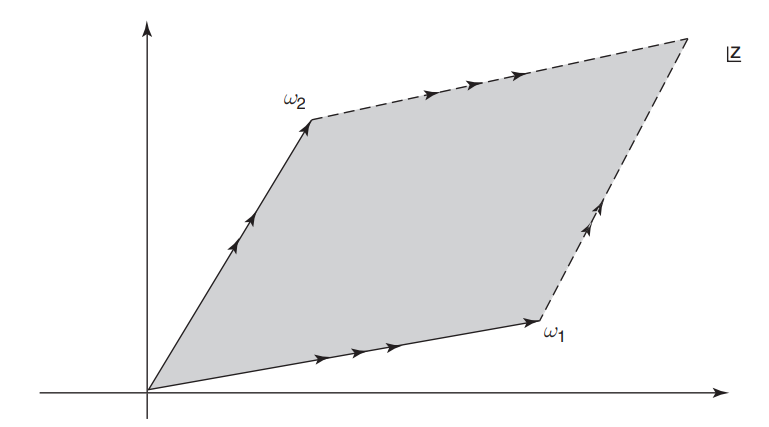
\includegraphics[width = 0.45\textwidth]{elements/general torus.PNG}
	\end{figure}
\end{frame}

\begin{frame}{\underline{Twisting the torus}}
	Intuitively, if a cylinder is twisted and the end surfaces are connected, we expect a different torus. 
	\\
	\underline{Formally}: Consider $\Re(\tau) \neq 0$ and a point $P = 0 = \tau$. We can reconstruct the rectangular $\textit{fundamental domain}$ by using the identification $z \sim z + 1$.
	\\
	\underline{Graphically}:
	\begin{figure}[htbp]
		\centering
		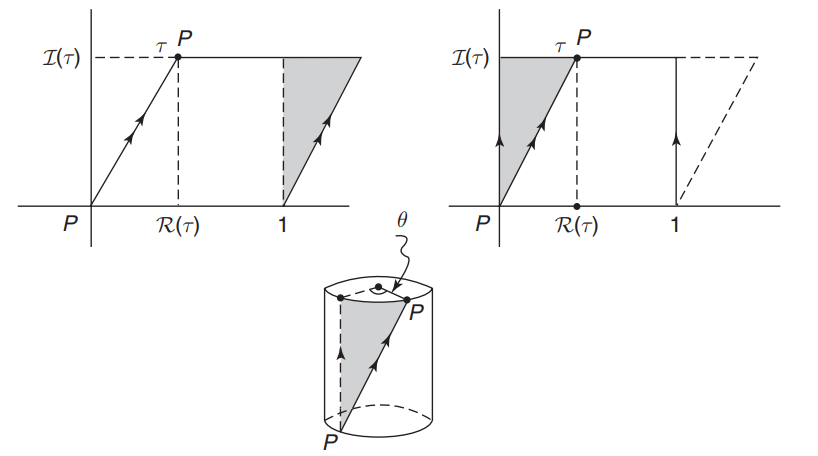
\includegraphics[width = 0.55\textwidth]{elements/twisted torus.PNG}
	\end{figure}
	
\end{frame}

\begin{frame}{\underline{Twisting parameter}}

	
	The point $P$ is no longer identified with a point on the perpendicular. Indeed the degree of twisting is parametrised by $\theta = 2\pi \Re(\tau)$.
	How does the twisting angle $\theta$ affect the torus parameter $\tau$?
	\\~\\
	Consider the map $\tau \rightarrow \tau + 1$:
	\begin{figure}[htbp]
		\centering
		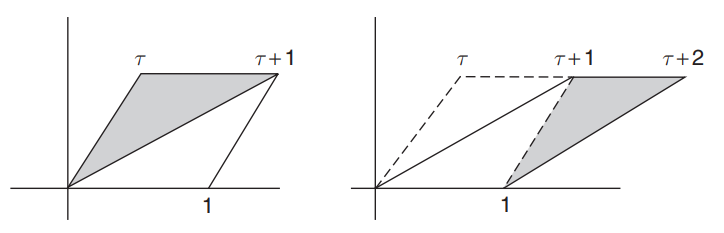
\includegraphics[width = 0.55\textwidth]{elements/tau map.PNG}
	\end{figure}
	With the identification $z \sim z + 1$ we can conclude $\tau \sim \tau + 1$ and hence $\theta \sim \theta + 2\pi$.
	\begin{block}{Note:}
		The "twisting" does not correspond to actual torsion. It is the mere identification of the points $P$.
	\end{block}
\end{frame}

\subsection{Fundamental domain}
\begin{frame}{\underline{Moduli space I}}
	So far we have established that $\Im(\tau) > 0 \Leftrightarrow \tau \in \mathbb{H}$.
	However, the identification $\tau \sim \tau + 1$ implies that the space of inequivalent tori is smaller. Indeed:
	\begin{block}{Strip $\mathcal{S}_{0}$}
		$\mathcal{S}_{0} = \{-\frac{1}{2} < \Re(\tau) < \frac{1}{2}, \Im(\tau) > 0\}$
	\end{block}
	Is $\mathcal{S}_{0}$ the moduli space of tori?
	\\
	For rectangular tori we found that $T, \frac{1}{T}$ yield equivalent tori. Since $\tau = iT$ we have $\tau' = \frac{i}{T} = -\frac{1}{\tau}$.
	\begin{figure}[htbp]
		\centering
		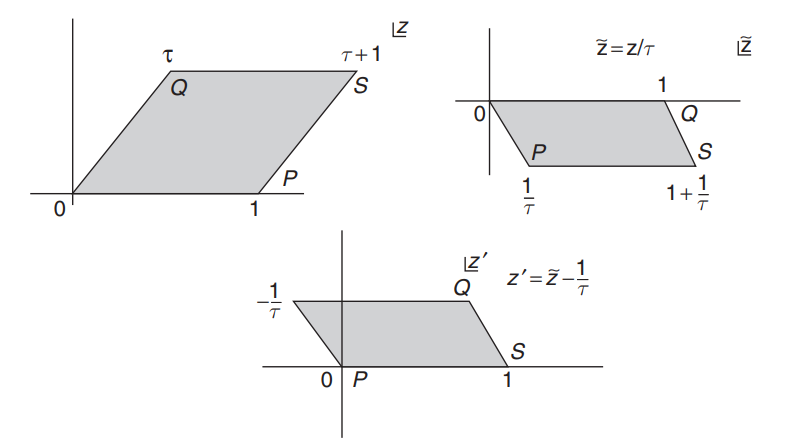
\includegraphics[width = 0.55\textwidth]{elements/s module trans.PNG}
	\end{figure}
\end{frame}

\begin{frame}{\underline{Moduli space II}}

	We have found two identifications with generators:
	\begin{block}{T-module transform}
		$T\tau = \tau + 1$
	\end{block}
	\begin{block}{S-module transform}
		$S\tau = -\frac{1}{\tau}$
	\end{block}
	The corresponding fundamental domain should be a subset of $\mathcal{S}_{0}$. Indeed, the S-module transform identifies points in $|\tau| < 1$ with points in $|\tau| > 1$.
	\\
	Therefore we can postulate:
	\begin{block}{Fundamental domain $\mathcal{F}_{0}$}
		$\mathcal{F}_{0} = \{-\frac{1}{2} < \Re(\tau) < \frac{1}{2}, \Im(\tau) > 0, |\tau| \geq 1 \textrm{ and } \Re(\tau) \geq 0 \textrm{ if } |\tau| = 1\}$
	\end{block}
	
\end{frame}


\begin{frame}

	% \begin{columns}
	% 	\begin{column}{0.25\textwidth}
	% 		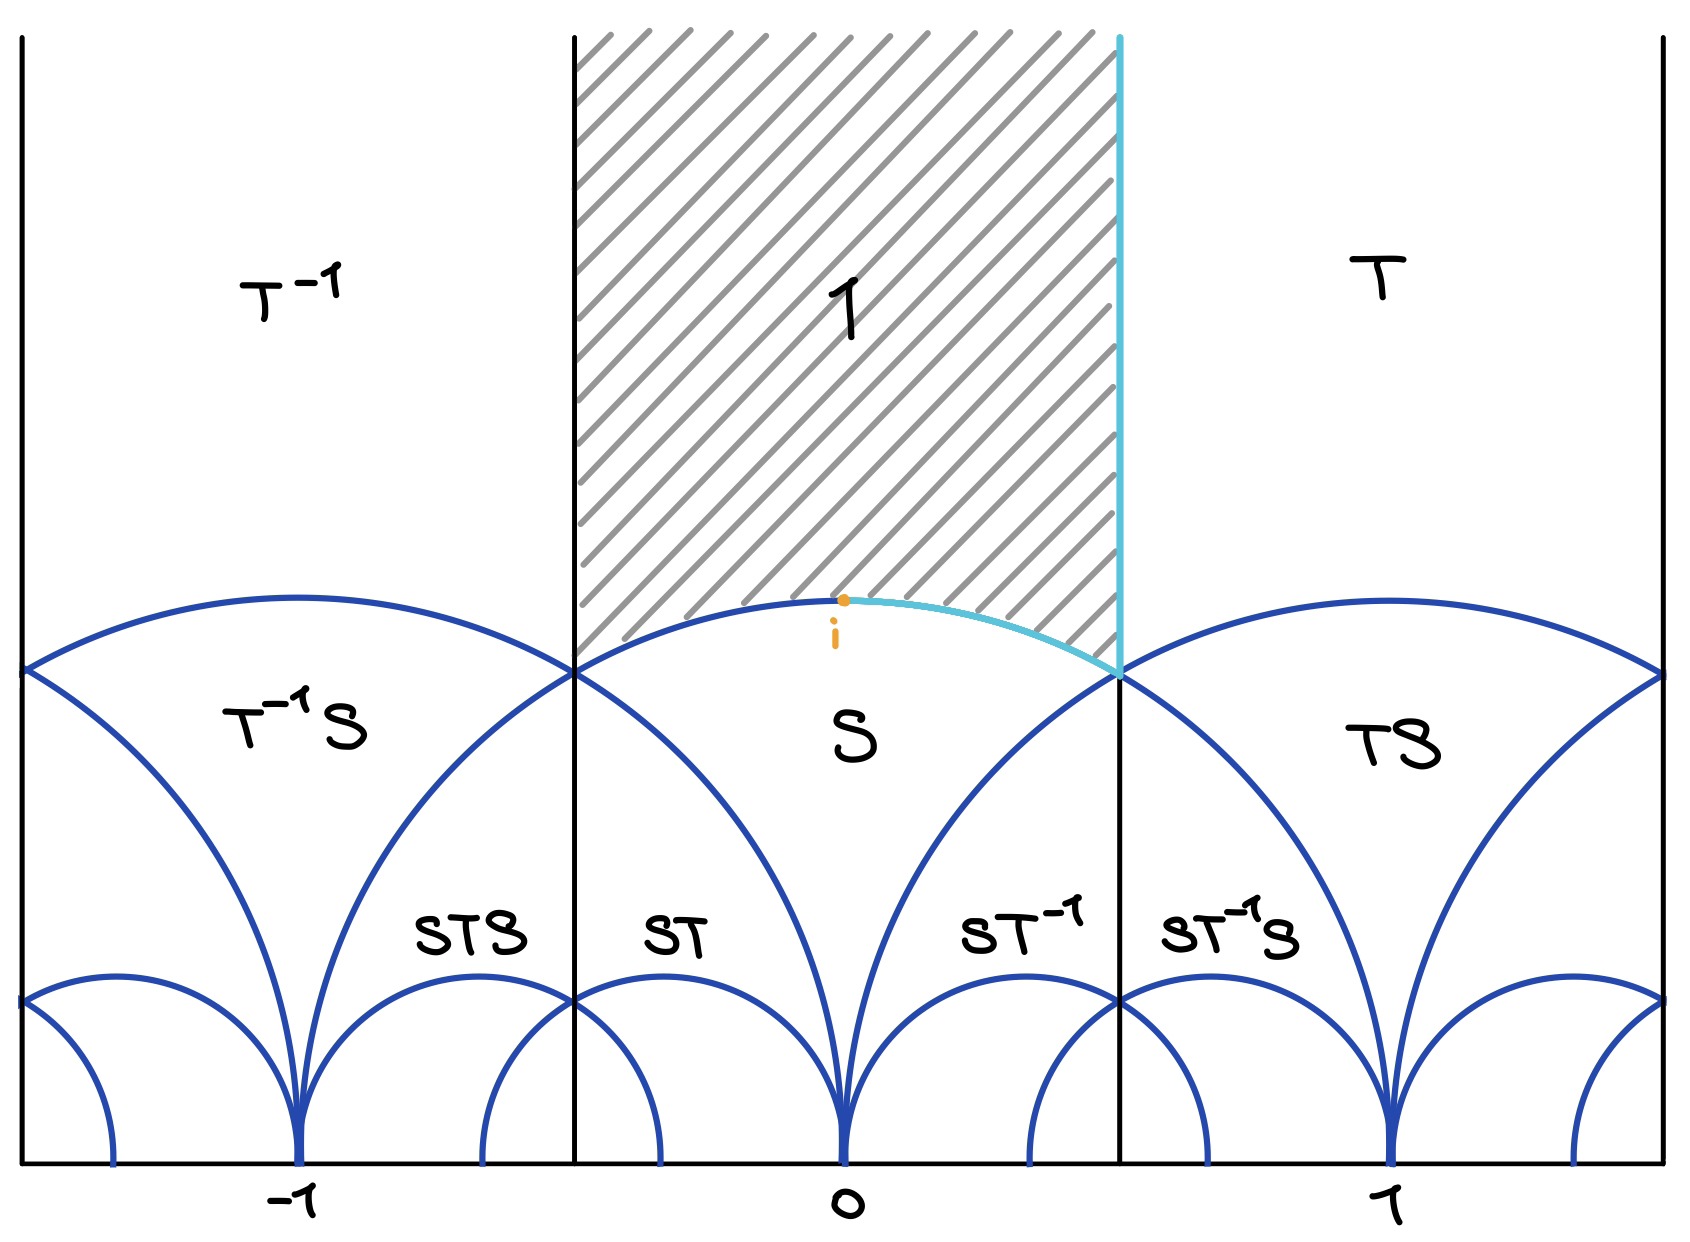
\includegraphics[width=\columnwidth]{elements/fundamental domain lucy.jpg}
	% 	\end{column}
	% 	\begin{column}{0.2\textwidth}
	% 		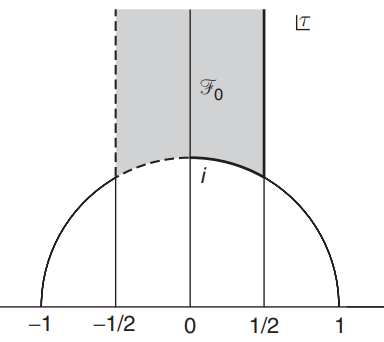
\includegraphics[width=\columnwidth]{elements/fundamental domain.PNG}
	% 	\end{column}
	% \end{columns}

	\begin{textblock*}{60mm}(0.05\paperwidth,0.25\paperheight)
		{\tiny \color{accentcolor}
		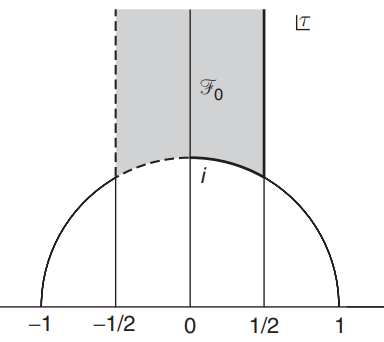
\includegraphics[width=60mm]{elements/fundamental domain.PNG}\\[2mm]
		}
	\end{textblock*}
	\begin{textblock*}{60mm}(0.45\paperwidth,0.32\paperheight)
		{\tiny \color{accentcolor}
		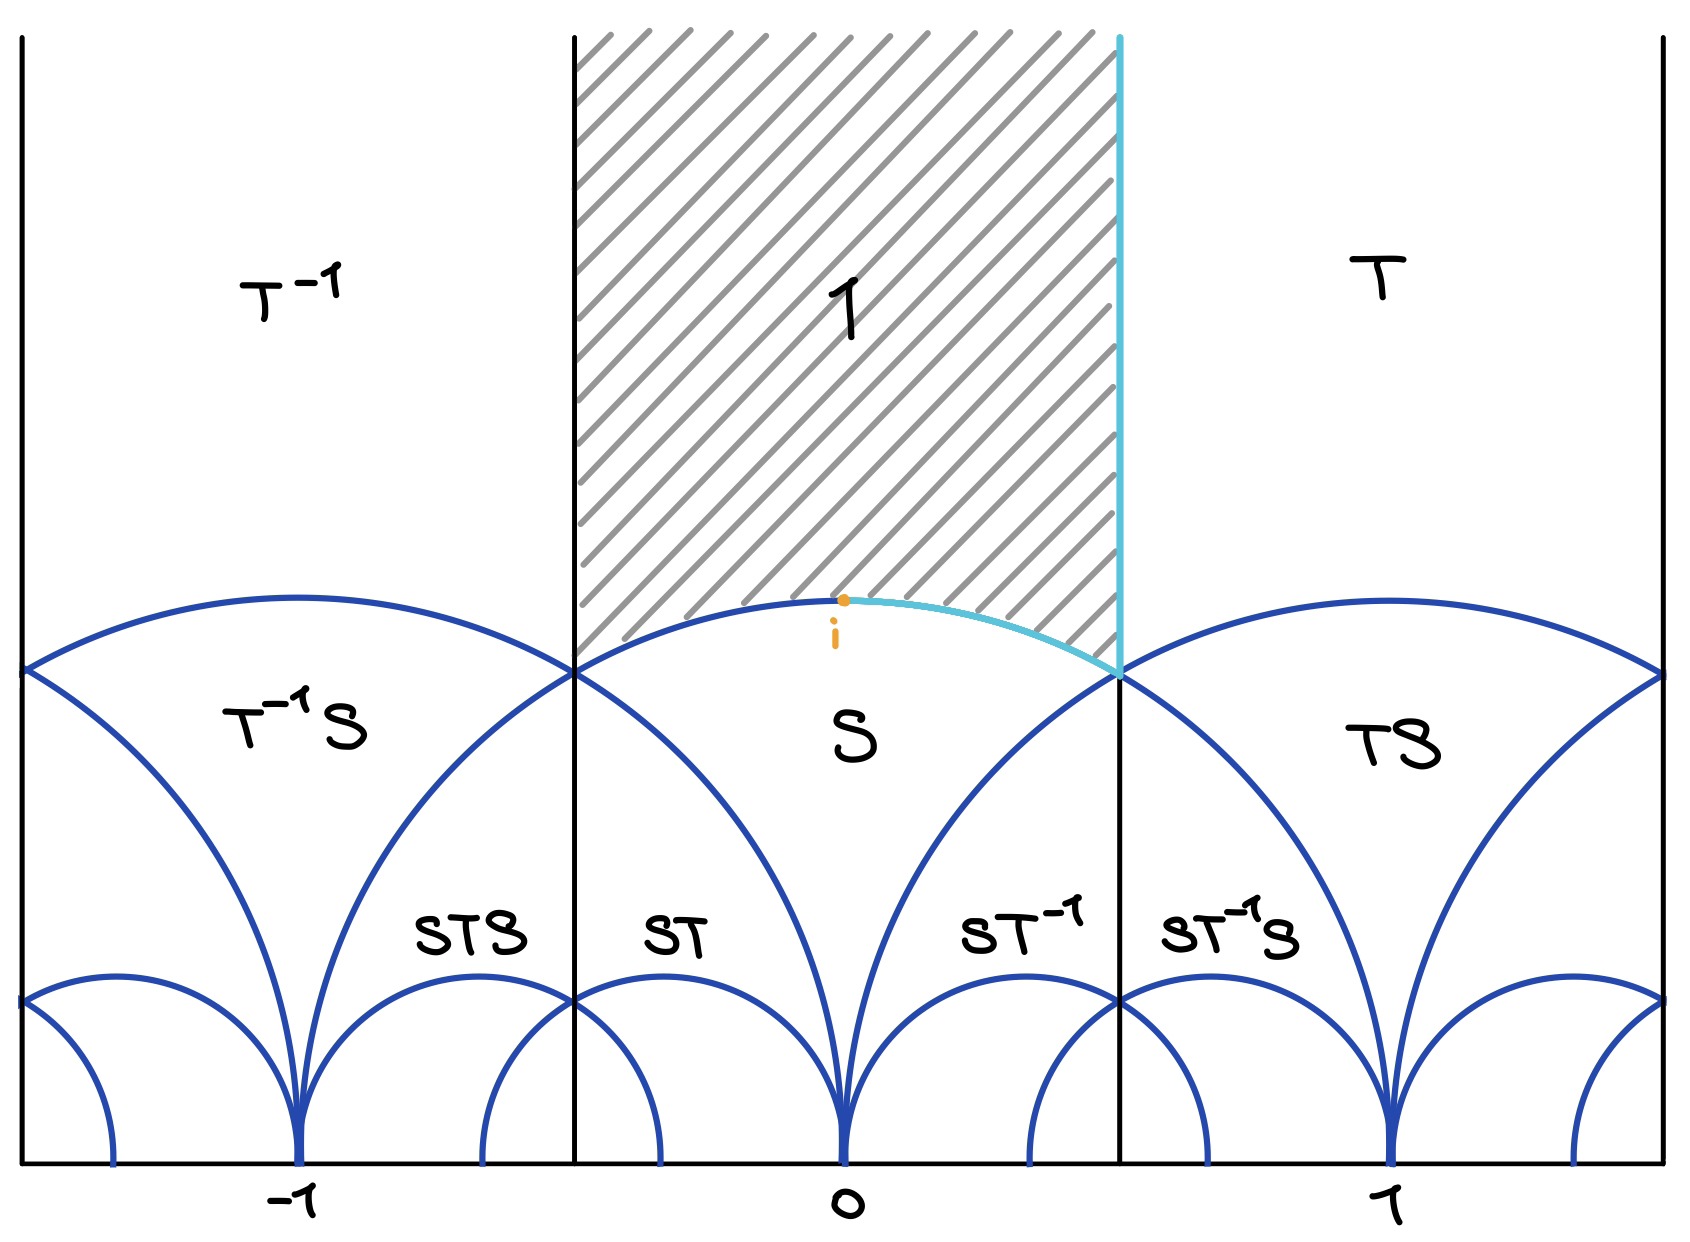
\includegraphics[width=60mm]{elements/fundamental domain lucy.jpg}\\[2mm]
		}
	\end{textblock*}

	
\end{frame}

\begin{frame}{\underline{Modular group $PSL(2, \mathbb{Z})$}}
	Consider a general linear fractional transformation $g \in G$:
	\begin{equation}
		g\tau = \frac{a\tau + b}{c\tau + d},~\Im(g\tau) = \frac{\Im(\tau)}{|c\tau + d|^2}
	\end{equation}
	with $a, b, c, d \in \mathbb{Z}$ and $ad- bc = 1$.
	\\
	Equivalently we can use a matrix representation:
	\begin{equation}
		[g] = \begin{pmatrix}
			a & b \\
			c & d \\
		\end{pmatrix},~\textrm{det}[g] = 1
	\end{equation}
	$\rightarrow$ $g$ satisfies the group homomorphism $\phi : G \rightarrow G$, $[g_1 g_2] \mapsto [g_1][g_2]$.
	\\
	We call $G$ the modular group $PSL(2, \mathbb{Z})$.
	\\~\\
	In matrix notation we see that $[T] = \big(\begin{smallmatrix}
		1 & 1\\
		0 & 1
	  \end{smallmatrix}\big)$ and $[S] = \big(\begin{smallmatrix}
		0 & -1\\
		1 & 0
	  \end{smallmatrix}\big)$ 
\end{frame}

\begin{frame}{\underline{Proving $\mathcal{F}_0$}}
	\begin{block}{Claim}
		For all $\tau \in \mathbb{H}$ exists $g \in G'$ such that $g\tau \in \mathcal{F}_0$
		\\
		$\rightarrow$ $\mathcal{F}_0$ contains exactly one copy of each inequivalent torus.
	\end{block}
	\underline{Step 1}: For each $\tau$ there is $g \in G'$ such that $\Im(g\tau)$ is largest.
	\\
	\underline{Step 2}: Show that $\tau' = T^{n}g\tau \in \mathcal{S}_0$ really is in $\bar{\mathcal{F}_0}$.
	\\
	\underline{Step 3}: Send $\tau \in \bar{\mathcal{F}_0}$ to $\tau \in \mathcal{F}_0$ via T- or S-transform.
\end{frame}

\section{Torus partition function}



\subsection{Compactified and Minkowsi closed strings}

\begin{frame}{Compactified bosonic string}
	Consider one compactified coordinate $X \sim X + 2\pi r$. In a free field theory the action can be written as 
	$S = \frac{1}{2\pi}\int \partial X \bar{\partial X}$ 
	\\
	For such coordinates the boundary conditions read:
	\begin{block}{BC}
		$X_0(z + \tau, \bar{z + \tau}) = X_0(z, \bar{z}) + 2\pi r n'$ 
		\\
		and 
		\\
		$X_0(z + 1, \bar{z + 1}) = X_0(z, \bar{z}) + 2\pi r n$
	\end{block}
	The solution to the classical equations of motion reads:
	\begin{equation}
		X_0^{(n, n')}(z, \bar{z}) = \frac{2\pi r}{2i\tau_2}(n'(z - \bar{z}) + n(\tau\bar{z} - \bar{\tau}z))
	\end{equation}
	$\rightarrow$ one dimension is compactified

\end{frame}


\begin{frame}{\underline{Partition function}}

	Obtaining the space-time form: 
	\begin{equation}
		p_L = \frac{m}{2r} + nr \textrm{ and }
		p_R = \frac{m}{2r} - nr
	\end{equation}
	For $r \rightarrow \infty$ we get continuous momenta $p_L = p_R = \frac{m}{2r}$.

	For a compactified closed string:
	\begin{equation}
		Z(r) = \int e^{-S} = \frac{1}{|\eta|^2} \sum_{m, n} q^{\frac{1}{2}p_L^2}\bar{q}^{\frac{1}{2}p_R^2}
	\end{equation}
	
	
\end{frame}
\begin{frame}{Return to Minkowski space}
	For $r \rightarrow \infty$ with $q = e^{2\pi i \tau}$:
	\begin{align*}
		Z(r) &= \frac{1}{|\eta|^2} \int_{-\infty}^{\infty}dk q^{\frac{1}{2}k^2}\bar{q}^{\frac{1}{2}} \\
		&= \frac{1}{|\eta|^2} \int_{-\infty}^{\infty}dk e^{2\pi i \frac{1}{2}k^2 \tau}e^{-2\pi i \frac{1}{2}k^2 \bar{\tau}} \\
		&= \frac{1}{|\eta|^2} \int_{-\infty}^{\infty}dk e^{2\pi i \frac{1}{2}k^2 2 i \Im{\tau}} \\
		&= \frac{1}{|\eta|^2} \int_{-\infty}^{\infty}dk e^{-2\pi k^2 \Im{\tau}} \\
		&\propto \frac{1}{|\eta|^2} \frac{1}{\Im(\tau)^{\frac{1}{2}}}
	\end{align*}
	
\end{frame}



\subsection{T-duality}

\begin{frame}{T-duality}
	Consider again the momentum and winding for the compactified string:
	\begin{equation}
		p = \frac{m}{r} \textrm{ and } w = nr
	\end{equation}
	We see that if we interchange $m \rightarrow n$ and $\frac{1}{r} \rightarrow r$, we interchange the meaning of winding and momentum. 
	\\
	This change however leaves the partition function invariant and we conclude T-duality.
\end{frame}




\subsection{Partition function via state trace}

\begin{frame}{Partition function via state trace}
	In quantum statistics:
	\begin{equation}
		Z = \Tr(e^{-\beta H}) \propto \sum_{\Phi}\bra{\Phi} H \ket{\Phi}
	\end{equation}
	The trace should run over all states of the torus. This means we need to find a propagator 
	which propagates through all configurations in $\tau$ and $\sigma$.
	Lets postulate:
	\begin{equation}
		Z(\tau) \propto \Tr(q^{L_0}\bar{q}^{\bar{L_0}})
	\end{equation} 
	with $q = e^{2\pi i \tau}$ and $L_0 = \sum \alpha_{-m}\alpha_m + \frac{1}{2}p_L^2$.
	

\end{frame}

\begin{frame}
	Is this a reasonable approach? Two hints:
	\\~\\
	I:
	\begin{equation}
		\Tr(q^{L_0}) \propto \Tr(q^{\sum_{n=1}^{\infty}\alpha_{-n}\alpha_n}) = \prod_{n=1}^{\infty}(1 + q^n + q^{2n} + \dots) = \prod_{n=1}^{\infty}\frac{1}{1-q^n}	
	\end{equation}
	This is the partition function of a boson from the Bose-Einstein distribution.
	\\~\\
	II:
	\begin{align*}
		q^{L_0}\bar{q}^{\bar{L_0}} &= e^{2\pi i (\tau_1 + i \tau_2)L_0}e^{-2\pi i (\tau_1 - i \tau_2)\bar{L_0}}\\
		&= e^{2 \pi i \tau_1 (L_0 - \bar{L_0})}e^{-2\pi \tau_2 (L_0 + \bar{L_0})}
	\end{align*}
	We can interpret $L_0 - \bar{L_0}$ as the momentum $P$ which generates translation in $\sigma$. Similarly $L_0 + \bar{L_0}$ can be seen as Hamiltonian $H$ which generates $\tau$ translation.
	\\
	The propagator has then the interpretation of a $\tau$ and $\sigma$ sweep.

\end{frame}

\begin{frame}
	The $\textit{Dedekind eta function}$ is defined as:
	\begin{equation}
		\eta(\tau) = q^{\frac{1}{24}}\prod_{n=1}^{\infty}(1 - q^n)
	\end{equation}
	Therefore we get:
	\begin{equation}
		(q\bar{q})^{-\frac{1}{24}}\Tr(q^{L_0}\bar{q}^{\bar{L_0}}) = \frac{1}{|\eta|^2}
	\end{equation}
	
\end{frame}


\section{Modular invariance of the amplitude}

\begin{frame}{\underline{The amplitude}}
	The correctly normalized one-loop vacuum amplitude reads:
	\begin{equation}
		A_0^{g=1} = \frac{V_{26}}{l_s^{26}}\int_{\mathcal{F}_0}\frac{d^2\tau}{4(\Im(\tau))^2}Z(\tau, \bar{\tau})
	\end{equation}
	This amplitude is carries the correct physical intuition: each possible form of a one-loop interaction is parametrised by $\tau$.
	To get a probability measure for a process we therefore need to weight every $\tau \in \mathcal{F}_0$ with the partition function $Z(\tau, \bar{\tau})$
	\\~\\
	The partition function for the 24-dimensional transverse coordinate space is:
	\begin{equation}
		Z(\tau, \bar{\tau}) = (\Im(\tau))^{-12}|\eta(\tau)|^{-48}
	\end{equation}
\end{frame}

\begin{frame}{\underline{Modular invariance}}
	The proposed amplitude is only valid if equivalent tori, i.e. equivalent interactions, result in the same amplitude. 
	\\
	We therefore need to have invariance under T- and S-module transforms.
	\\
	The integration domain $\mathcal{F}_0$ is by definition modular invariant. 
	\\
	Consider a general modular transformation $g$ on the measure:
	\begin{align*}
		d(g\tau) &=  [\frac{a(c\tau + d) - (a\tau + b)c}{(c\tau + d)^2}]d\tau \\
		&= [\frac{ad - bc}{(c\tau + d)^2}]d\tau
	\end{align*}
	So $d^2\tau \rightarrow |c\tau + d|^{-4}d^2\tau$
	\\
	Also: $\Im(\tau) \rightarrow |c\tau + d|^{-2}\Im(\tau)$
	
\end{frame}











\end{document}